% !TEX encoding = UTF-8 Unicode
\documentclass[a4paper]{article}

\usepackage{color}
\usepackage{url}
\usepackage[T2A]{fontenc} % enable Cyrillic fonts
\usepackage[utf8]{inputenc} % make weird characters work
\usepackage{graphicx}
\usepackage[section]{placeins}

\usepackage[english,serbian]{babel}
%\usepackage[english,serbianc]{babel} %ukljuciti babel sa ovim opcijama, umesto gornjim, ukoliko se koristi cirilica

\usepackage[unicode]{hyperref}
\hypersetup{colorlinks,citecolor=green,filecolor=green,linkcolor=blue,urlcolor=blue}

\usepackage{listings}
\usepackage{subfiles}

\usepackage{tabularx}
\usepackage{longtable}

%\newtheorem{primer}{Пример}[section] %ćirilični primer
\newtheorem{primer}{Primer}[section]

\definecolor{mygreen}{rgb}{0,0.6,0}
\definecolor{mygray}{rgb}{0.5,0.5,0.5}
\definecolor{mymauve}{rgb}{0.58,0,0.82}

\lstset{ 
  backgroundcolor=\color{white},   % choose the background color; you must add \usepackage{color} or \usepackage{xcolor}; should come as last argument
  basicstyle=\scriptsize\ttfamily,        % the size of the fonts that are used for the code
  breakatwhitespace=false,         % sets if automatic breaks should only happen at whitespace
  breaklines=true,                 % sets automatic line breaking
  captionpos=b,                    % sets the caption-position to bottom
  commentstyle=\color{mygreen},    % comment style
  deletekeywords={...},            % if you want to delete keywords from the given language
  escapeinside={\%*}{*)},          % if you want to add LaTeX within your code
  extendedchars=true,              % lets you use non-ASCII characters; for 8-bits encodings only, does not work with UTF-8
  firstnumber=1000,                % start line enumeration with line 1000
  frame=single,	                   % adds a frame around the code
  keepspaces=true,                 % keeps spaces in text, useful for keeping indentation of code (possibly needs columns=flexible)
  keywordstyle=\color{blue},       % keyword style
  language=Python,                 % the language of the code
  morekeywords={*,...},            % if you want to add more keywords to the set
  numbers=left,                    % where to put the line-numbers; possible values are (none, left, right)
  numbersep=5pt,                   % how far the line-numbers are from the code
  numberstyle=\tiny\color{mygray}, % the style that is used for the line-numbers
  rulecolor=\color{black},         % if not set, the frame-color may be changed on line-breaks within not-black text (e.g. comments (green here))
  showspaces=false,                % show spaces everywhere adding particular underscores; it overrides 'showstringspaces'
  showstringspaces=false,          % underline spaces within strings only
  showtabs=false,                  % show tabs within strings adding particular underscores
  stepnumber=2,                    % the step between two line-numbers. If it's 1, each line will be numbered
  stringstyle=\color{mymauve},     % string literal style
  tabsize=2,	                   % sets default tabsize to 2 spaces
  title=\lstname                   % show the filename of files included with \lstinputlisting; also try caption instead of title
}
\begin{document}

\title{Informacioni sistem za teretane\\ \small{Seminarski rad u okviru kursa\\Informacioni sistemi\\ Matematički fakultet}}

\author{Selena Vukadinović (1070/2020) mi15088@alas.matf.bg.ac.rs ,\\ Tamara Ivanović (1108/2020) mi14262@alas.matf.bg.ac.rs,\\ Jana Jovičić (1097/2019) mi15215@alas.matf.bg.ac.rs, \\Jovana Pejkić (1089/2020), \\ Katarina Đurić (1069/2020) mr14236@alas.matf.bg.ac.rs}

%\date{9.~april 2015.}

\maketitle


\vfill

\begin{flushleft}
Profesor:\\
\textbf{dr Saša Malkov}\\[.3cm] % Advisor's/supervisor's name
Asistent:\\
\textbf{Anja Bukurov}\\[.3cm] % Tutor's name
\end{flushleft}

\newpage

\tableofcontents
\newpage


% Uvod
\section{Uvod}
\label{sec:uvod}
\subfile{sections/uvod}


% DTP
\section{Dijagrami toka podataka}
\subfile{sections/dijagrami_toka_podataka}


% Slucajevi upotrebe
\section{Slučajevi upotrebe}


% Neregistrovani korisnik
\subsection{Aktivnosti neregistrovanog korisnika}
\begin{figure}[!ht]
\begin{center}
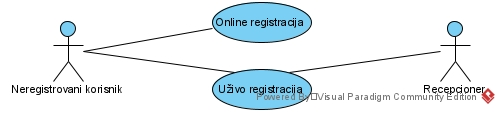
\includegraphics[scale=0.55]{sections/images/dijagram_slucajeva_upotrebe_neregistrovanog_korisnika.jpg}
\end{center}
\caption{Dijagram slučajeva upotrebe neregistrovanog korisnika}
\label{fig:kontekst}
\end{figure}

\subsubsection{Slučaj upotrebe: Registracija korisnika uživo}
\subfile{sections/korisnik/uzivo_registracija}

\subsubsection{Slučaj upotrebe: Registracija online}
\subfile{sections/korisnik/registracija_neregistrovanog_korisnika}
\newpage
\begin{figure}[!ht]
\begin{center}
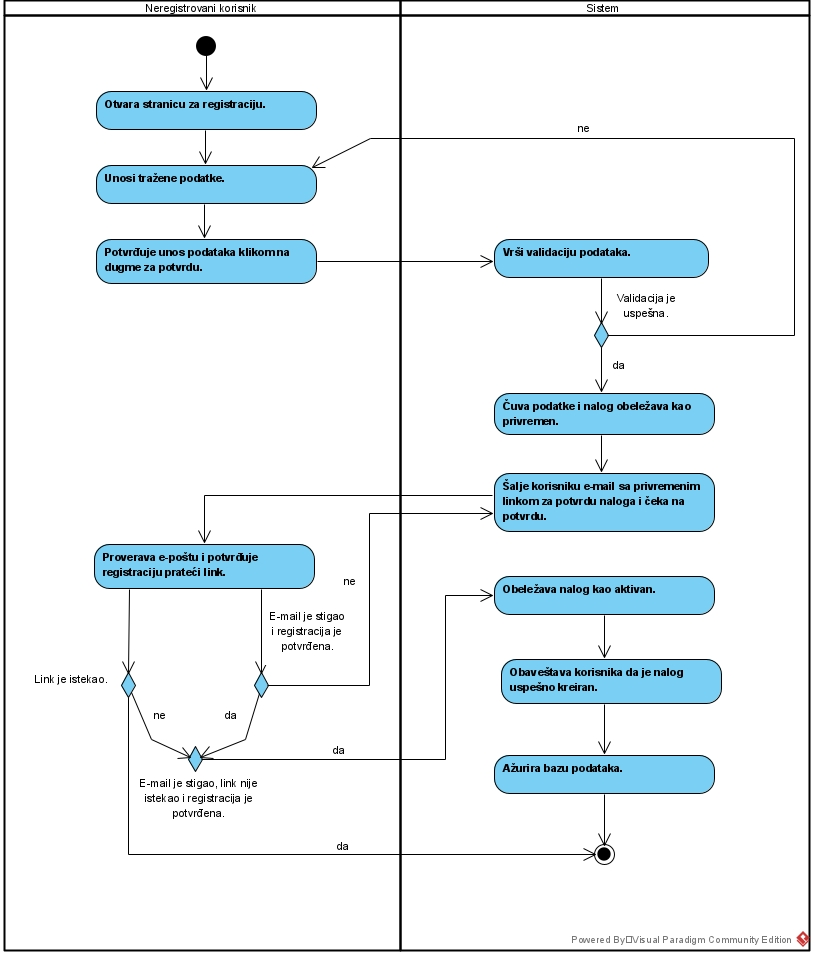
\includegraphics[scale=0.50]{sections/images/dijagram_aktivnosti_registracija_neregistrovanog_korisnika_online.jpg}
\end{center}
\caption{Dijagram aktivnosti za online registraciju neregistrovanog korisnika}
\label{fig:kontekst}
\end{figure}


% Klijent
\newpage
\subsection{Aktivnosti klijenta}
\begin{figure}[!ht]
\begin{center}
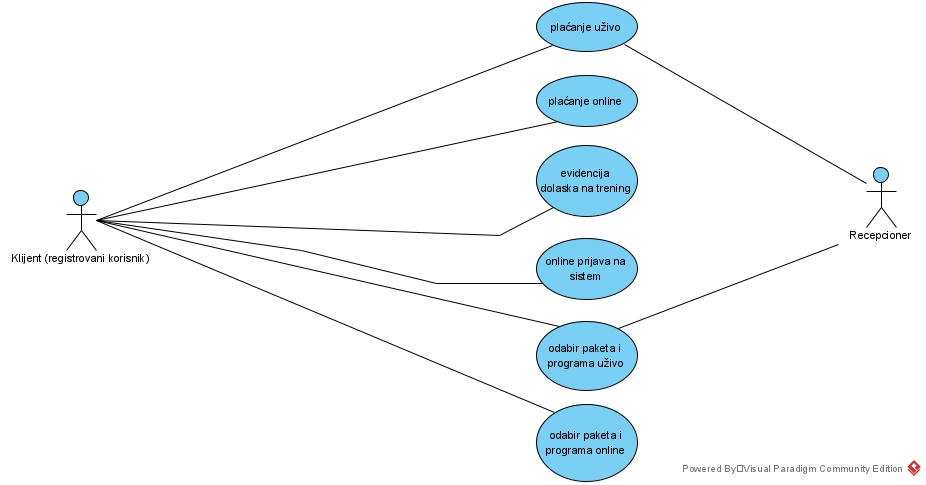
\includegraphics[scale=0.45]{sections/images/dijagram_slucajeva_upotrebe_klijenta.jpg}
\end{center}
\caption{Dijagram slučajeva upotrebe klijenta}
\label{fig:kontekst}
\end{figure}

\subsubsection{Slučaj upotrebe: Plaćanje članarine uživo}
\subfile{sections/korisnik/placanje_uzivo}

\subsubsection{Slučaj upotrebe: Online plaćanje za klijenta}
\subfile{sections/korisnik/online_placanje_za_registrovanog_korisnika}
\begin{figure}[!ht]
\begin{center}
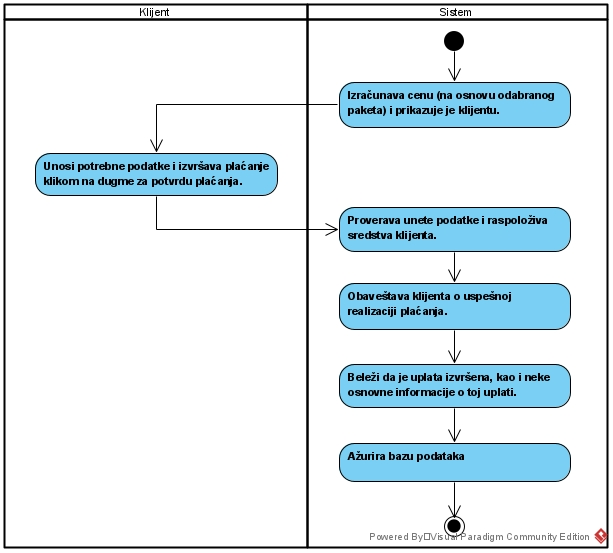
\includegraphics[scale=0.40]{sections/images/dijagram_aktivnosti_za_online_placanje_klijenta.jpg}
\end{center}
\caption{Dijagram aktivnosti za online plaćanje klijenta}
\label{fig:kontekst}
\end{figure}

\subsubsection{Slučaj upotrebe: Evidencija dolaska na trening}
\subfile{sections/evidencija_prisustva}

\subsubsection{Slučaj upotrebe: Online prijava za klijenta}
\subfile{sections/korisnik/online_prijava_registrovanog_korisnika}
\begin{figure}[!ht]
\begin{center}
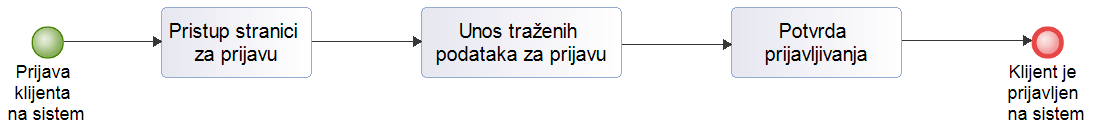
\includegraphics[scale=0.55]{sections/images/bpmn_dijagram_procesa_online_prijava_klijenta_na_sistem.png}
\end{center}
\caption{BPMN dijagram procesa za online prijavu klijenta}
\label{fig:kontekst}
\end{figure}

\subsubsection{Slučaj upotrebe: Odabir paketa i programa online}
\subfile{sections/korisnik/odabir_paketa_i_programa_online}
\begin{figure}[!ht]
\begin{center}
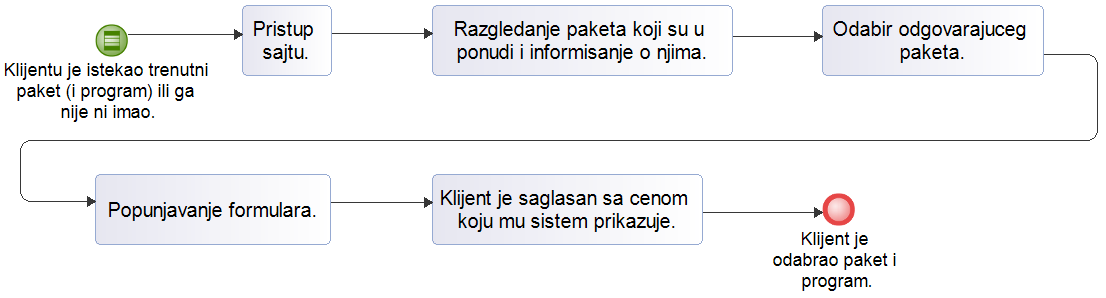
\includegraphics[scale=0.55]{sections/images/bpmn_dijagram_procesa_odabir_paketa_i_programa_online.png}
\end{center}
\caption{BPMN dijagram procesa za online odabir paketa i programa}
\label{fig:kontekst}
\end{figure}

\subsubsection{Slučaj upotrebe: Odabir paketa i programa uživo}
\subfile{sections/korisnik/odabir_paketa_i_programa_uzivo}
\begin{figure}[!ht]
\begin{center}
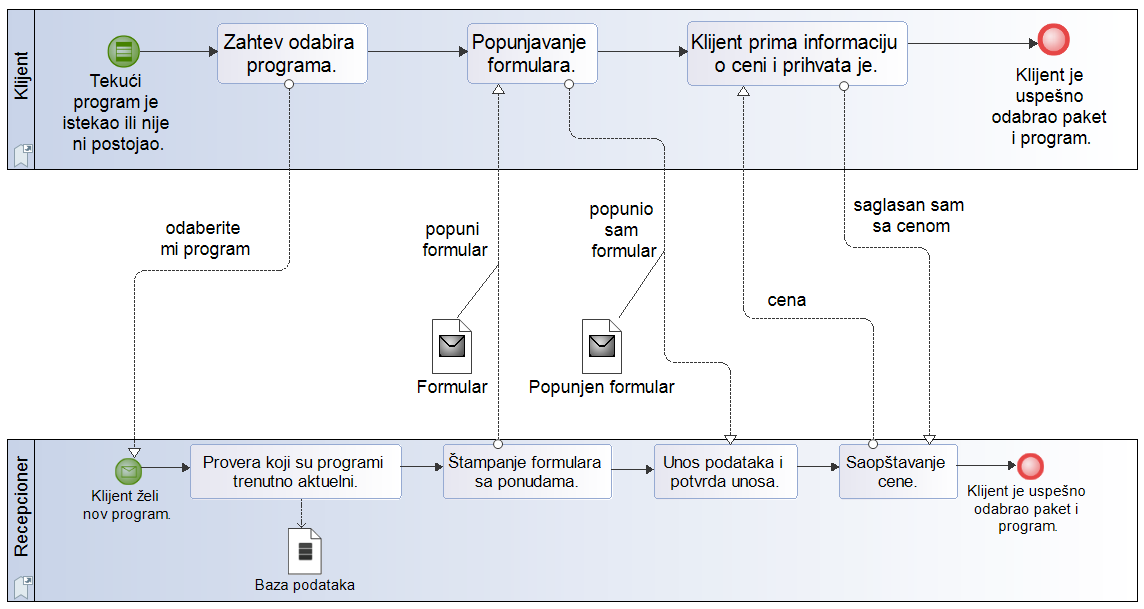
\includegraphics[scale=0.55]{sections/images/bpmn_dijagram_saradnje_odabir_paketa_i_programa_uzivo.png}
\end{center}
\caption{BPMN dijagram saradnje za odabir paketa i programa uživo}
\label{fig:kontekst}
\end{figure}


%%%%%%% Personalni treninzi
\newpage
\subsection{Aktivnosti vezane za personalne treninge}
\subfile{sections/personalni_treninzi}

%%%%%%% Grupni treninzi
\newpage
\subsection{Aktivnosti vezane za grupne treninge}
\subfile{sections/grupniTreninzi.tex}

%%%%%% administrator
\newpage
\subsection{Aktivnosti administratora}

\begin{figure}[!ht]
\begin{center}
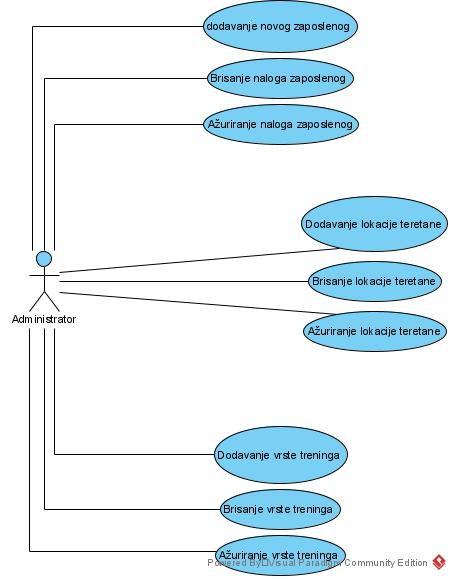
\includegraphics[scale=0.55]{sections/images/dijagram_slucajeva_upotrebe_administratora.jpg}
\end{center}
\caption{Dijagram slučajeva upotrebe administratora}
\label{fig:kontekst}
\end{figure}

\subsubsection{Slučaj upotrebe: Registracija novog zaposlenog}
\subfile{sections/administrator/registracija_zaposlenog}

\begin{figure}[!ht]
\begin{center}
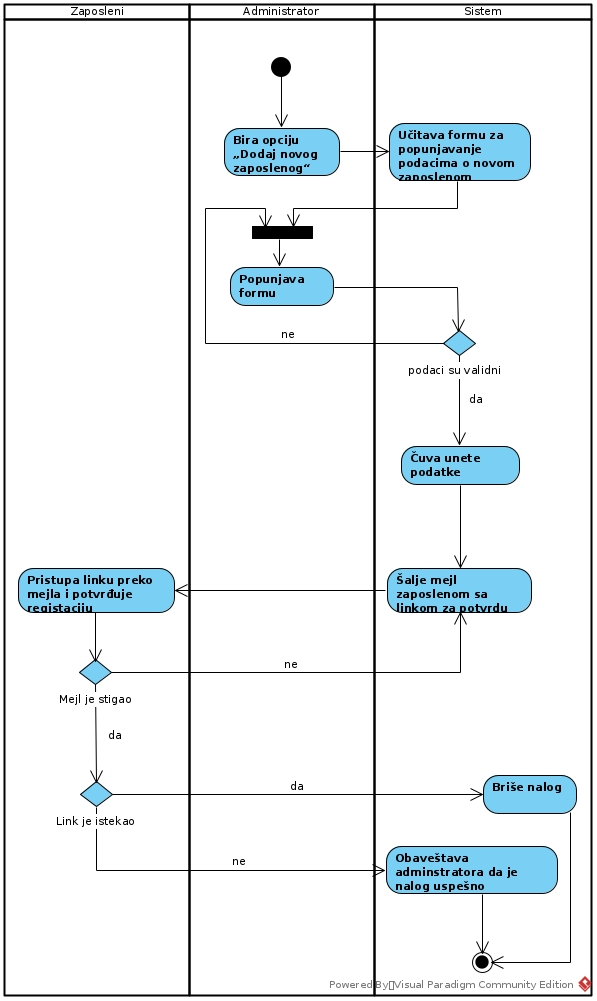
\includegraphics[scale=0.52]{sections/images/dijagram_aktivnosti_registracije_zaposlenog.jpg}
\end{center}
\caption{Dijagram aktivnosti registracije zaposlenog}
\label{fig:kontekst}
\end{figure}

\subsubsection{Slučaj upotrebe: Ažuriranje naloga zaposlenog}
\subfile{sections/administrator/azuriranje_naloga_zaposlenog}

\newpage
\begin{figure}[!ht]
\begin{center}
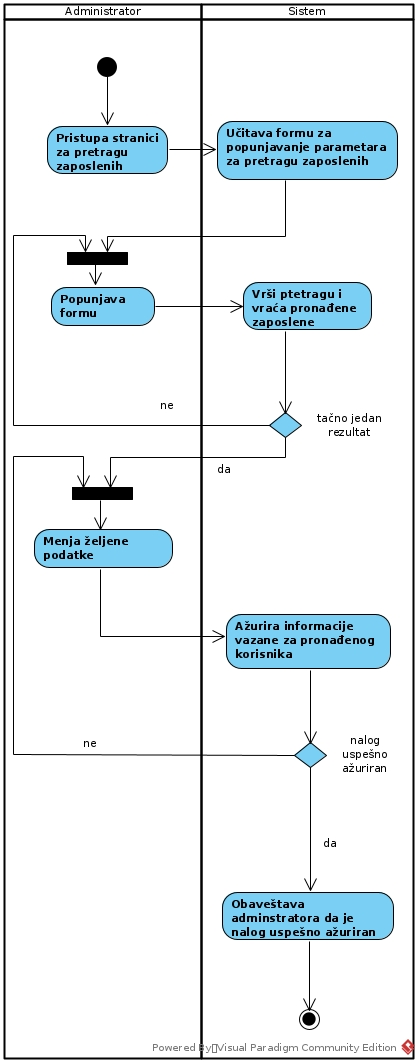
\includegraphics[scale=0.50]{sections/images/dijagram_aktivnosti_azuriranja_naloga_zaposlenog.jpg}
\end{center}
\caption{Dijagram aktivnosti ažuriranja naloga zaposlenog}
\label{fig:kontekst}
\end{figure}

\subsubsection{Slučaj upotrebe: Brisanje zaposlenog}
\subfile{sections/administrator/brisanje_naloga_zaposlenog}


\subsubsection{Slučaj upotrebe: Dodavanje nove lokacije}
\subfile{sections//administrator/nova_lokacija}

\subsubsection{Slučaj upotrebe: Ažuriranje lokacije}
\subfile{sections//administrator/azuriranje_lokacije}

\subsubsection{Slučaj upotrebe: Uklanjanje lokacije}
\subfile{sections//administrator/brisanje_lokacije}


\subsubsection{Slučaj upotrebe: Dodavanje vrste treninga}
\subfile{sections/administrator/nova_vrsta_treninga}

\subsubsection{Slučaj upotrebe: Ažuriranje vrste treninga}
\subfile{sections/administrator/azuriranje_vrste_treninga}

\subsubsection{Slučaj upotrebe: Brisanje vrste treninga}
\subfile{sections/administrator/brisanje_vrste_treninga}


%%%%%%%%%%%%%Takmičenje
\newpage
\subsection{Takmičenje}
Takmičenje predstavlja poseban slučaj upotrebe koji nije uvek aktivan. Ukoliko administrator zakaže novo takmičenje u informacionom sistemu se omogućava pristup prijavi. 

\begin{figure}[!ht]
\begin{center}
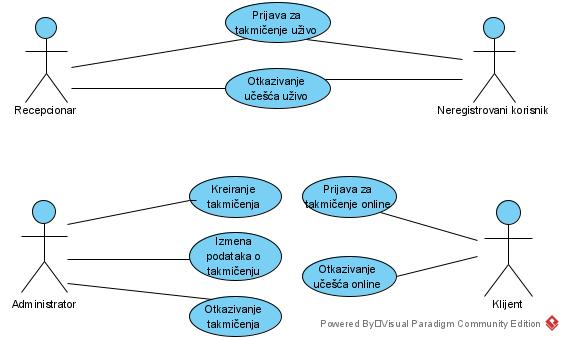
\includegraphics[scale=0.55]{sections/images/dijagram_slucajeva_upotrebe_za_takmicenje.jpg}
\end{center}
\caption{Dijagram slučajeva upotrebe za takmičenje}
\label{fig:kontekst}
\end{figure}

\subsubsection{Slučaj upotrebe: Kreiranje takmičenja}
\subfile{sections/takmicenje/kreiranje_takmicenja}

\subsubsection{Slučaj upotrebe: Prijava za takmičenje uživo}
\subfile{sections/takmicenje/prijava_takmicenje_uzivo}

\subsubsection{Slučaj upotrebe: Prijava za takmičenje online}
\subfile{sections/takmicenje/prijava_takmicenje_online}

\subsubsection{Slučaj upotrebe: Otkazivanje učešća uživo}
\subfile{sections/takmicenje/odustajanje_od_takmicenja_uzivo}

\subsubsection{Slučaj upotrebe: Otkazivanje učešća online}
\subfile{sections/takmicenje/odustajanje_od_takmicenja_online}

\subsubsection{Slučaj upotrebe: Izmena podataka o takmičenju}
\subfile{sections/takmicenje/izmena_takmicenja}

\subsubsection{Slučaj upotrebe: Otkazivanje takmičenja}
\subfile{sections/takmicenje/otkazivanje_takmicenja}


%%%%%%%%%%%%% Licenca
\newpage
\subsection{Licenca za trenera}

U okviru teretana se organizuju obuke za članove koji žele da postanu treneri, bilo personalni, bilo treneri grupnih programa. Ukoliko klijent ispunjava zahteve konkursa za obuku, može podneti potrebnu dokumentaciju i upisati se na odgovarajući program obuke. Nakon završetka obuke i položenih svih potrebnih testova, klijent dobija licencu za trenera i stiče mogućnost zaposlenja u teretani.

\begin{figure}[!ht]
\begin{center}
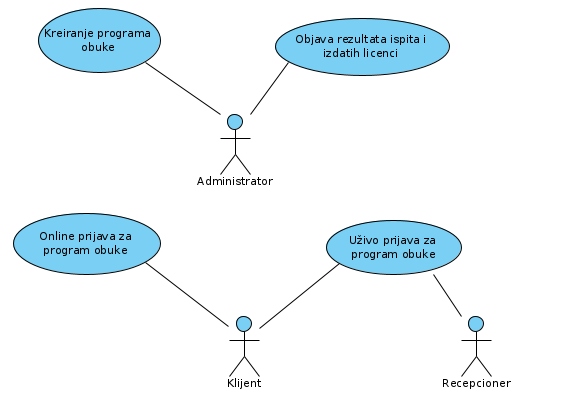
\includegraphics[scale=0.55]{sections/images/slucajevi_upotrebe_za_licencu.png}
\end{center}
\caption{Dijagram slučajeva upotrebe za program obuke za licencu}
\label{fig:kontekst}
\end{figure}


\subsubsection{Slučaj upotrebe: Kreiranje programa obuke}
\subfile{sections/licenca/kreiranje_programa_obuke}

\subsubsection{Slučaj upotrebe: Online prijava za program obuke}
\subfile{sections/licenca/online_prijava_za_program_obuke}

\subsubsection{Slučaj upotrebe: Uživo prijava za program obuke}
\subfile{sections/licenca/uzivo_prijava_za_program_obuke}

\subsubsection{Slučaj upotrebe: Objava rezultata ispita i izdatih licenci}
\subfile{sections/licenca/rezultati}


% Igraonica
\subsection{Igraonica}

\subsubsection{Slučaj upotrebe: Dodavanje nove igraonice u sistem}
\subfile{sections/decja_igraonica/dodavanje_nove_igraonice}
\begin{figure}[!ht]
\begin{center}
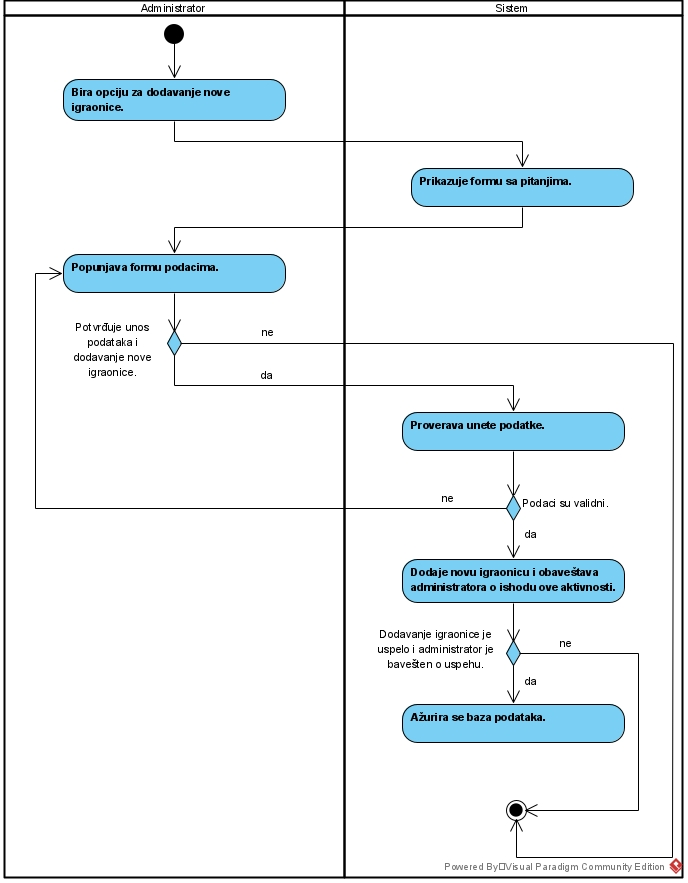
\includegraphics[scale=0.55]{sections/images/dijagram_aktivnosti_dodavanja_nove_igraonice.jpg}
\end{center}
\caption{Dijagram aktivnosti za dodavanje nove igraonice}
\label{fig:kontekst}
\end{figure}

\subsubsection{Slučaj upotrebe: Uklanjanje postojeće igraonice iz sistema}
\subfile{sections/decja_igraonica/uklanjanje_postojece_igraonice}
\begin{figure}[!ht]
\begin{center}
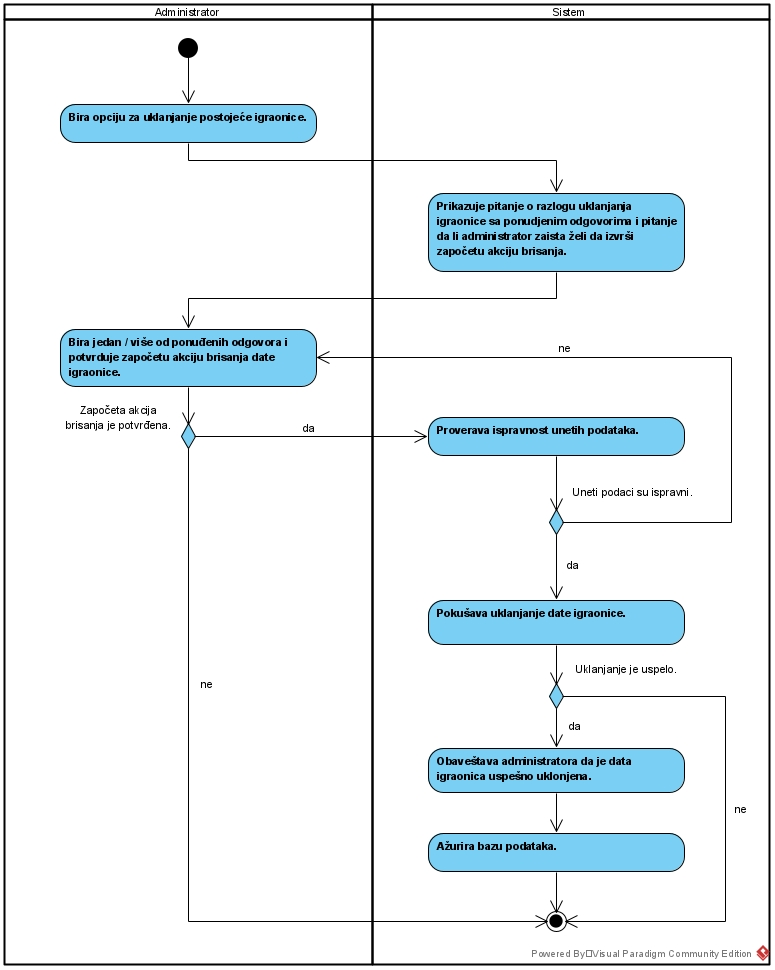
\includegraphics[scale=0.55]{sections/images/dijagram_aktivnosti_uklanjanje_postojece_igraonice.jpg}
\end{center}
\caption{Dijagram aktivnosti za uklanjanje postojeće igraonice}
\label{fig:kontekst}
\end{figure}

\subsubsection{Slučaj upotrebe: Evidencija dolaska u igraonicu}
\subfile{sections/decja_igraonica/evidencija_dolaska}

\subsubsection{Slučaj upotrebe: Usluge igraonice online}
\subfile{sections/decja_igraonica/usluga_igraonice_online}
\begin{figure}[!ht]
\begin{center}
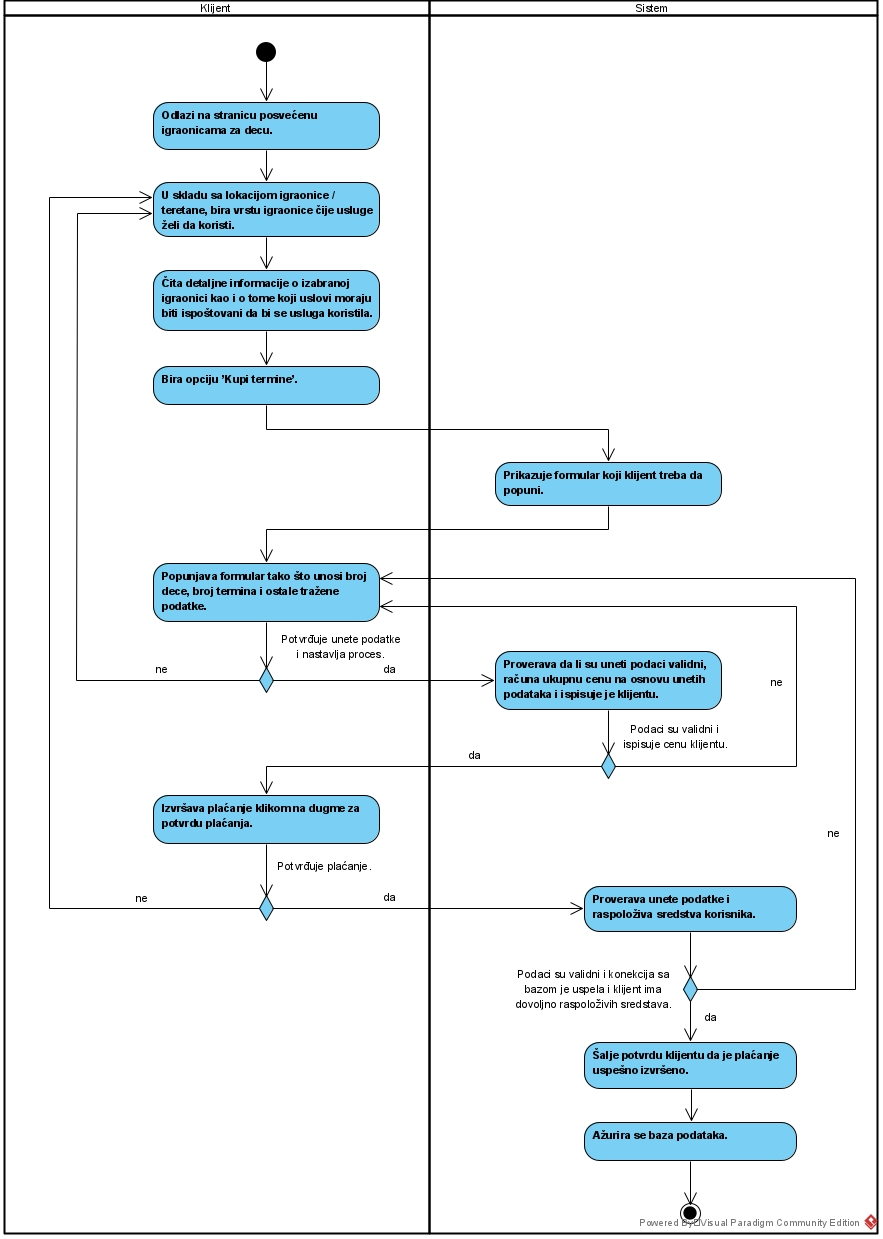
\includegraphics[scale=0.45]{sections/images/dijagram_aktivnosti_usluge_igraonice_online.jpg}
\end{center}
\caption{Dijagram aktivnosti za usluge igraonice online}
\label{fig:kontekst}
\end{figure}

\subsubsection{Slučaj upotrebe: Usluge igraonice uživo}
\subfile{sections/decja_igraonica/usluga_igraonice_uzivo}
\begin{figure}[!ht]
\begin{center}
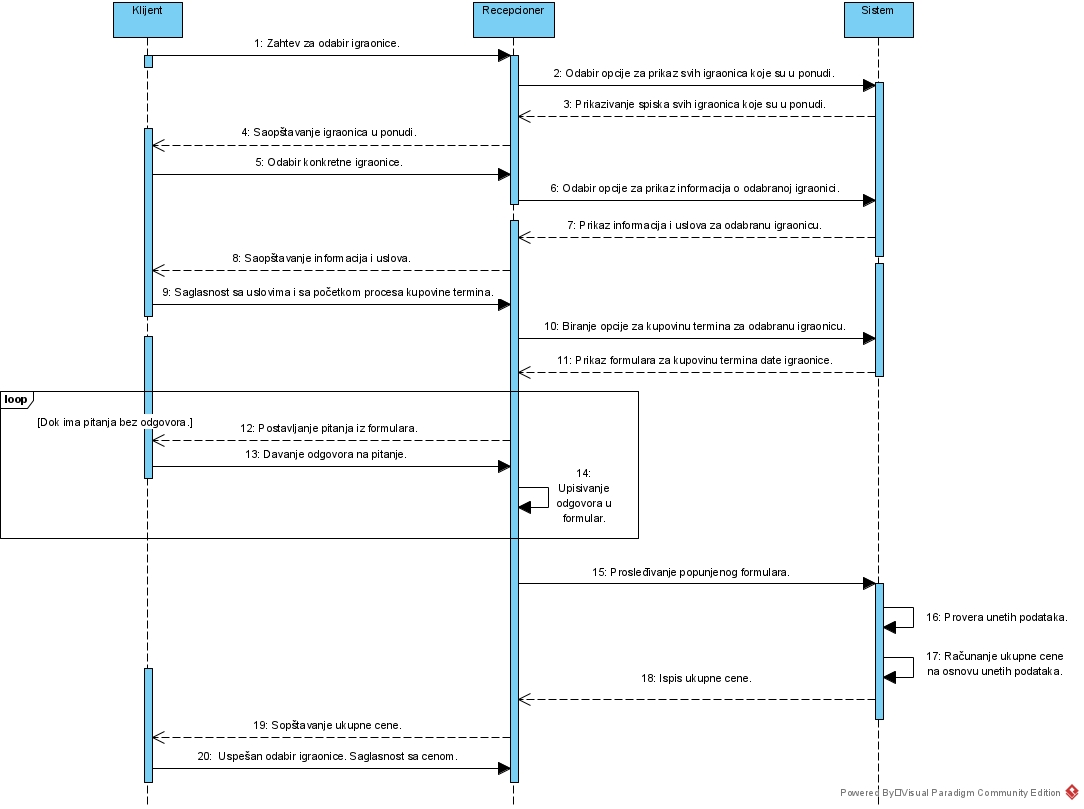
\includegraphics[scale=0.4]{sections/images/dijagram_sekvenci_usluge_igraonice_uzivo.jpg}
\end{center}
\caption{Dijagram sekvenci za usluge igraonice uživo}
\label{fig:kontekst}
\end{figure}

\newpage
\newpage
\newpage
\section{Opis baze podataka}
\subfile{sections/opis_baze_podataka}

\newpage
\section{Arhitektura sistema}
\subfile{sections/arhitektura_sistema}

\newpage
\section{Korisnički interfejs}
\subfile{sections/korisnicki_interfejs/korisnicki_interfejs}

\end{document}